\documentclass{UoYCSproject}
\usepackage{color,soul}
\usepackage{graphicx}
\usepackage{amsmath}
\usepackage{amssymb}

\addbibresource{refs.bib}

\author{Patrick Buhagiar}
\title{The Impact of Macroeconomic Parameters on Forecasting Financial Markets}
\date{2018-July-06}
\supervisor{Dimitar Kazakov}
\MIP
\wordcount{8832}

\includes{Appendices \ref{cha:usefulpackages}, \ref{cha:gotchas} and
  \ref{cha:deptfac}}

\excludes{\autoref{cha:quoteex}}

\abstract{ 
    Financial forecasting is a common area in machine learning, however a gap in literature was identified with respect to the influence of macroeconomic variables in predicting financial markets. This study attempts to use ensemble methods to predict the direction of the FTSE market in relation to other financial markets and macroeconomic variables in the UK. This study adopts a two-stage process. The first stage consists of creating several ANN models for different time periods that predict the stock market based on the closing prices of other markets. The second stage consists of feeding the results from the first stage and macroeconomic data into another ANN. \hl{TODO add result summary as last sentence}
}

\dedication{To all students everywhere}

\acknowledgements{To my cactus, that I forget to water}
\bibliography{refs}
\begin{document}

\maketitle

\listoffigures
\listoftables

\label{sec:start}
\thispagestyle{empty}\cleardoublepage

\chapter{Introduction}
\label{cha:introduction}



\chapter{Background}
\label{cha:background}

\section{The Relationship Between Macroeconomics and Microeconomics}
Economics can be divided into two branches of study: macroeconomics and microeconomics. Macroeconomics is the study of the behaviour, performance and trends of an economy as a whole \cite{2003economics}. Macro-economists evaluate a variety of economy-wide phenomena such as inflation, gross domestic product (GDP) and unemployment. To keep the economy in check, governments look at these factors to aid in economic policy decision making. Microeconomics on the other hand is the study of how individuals make economic decisions and their effect on the economy. These individuals are classified into consumers, producers and resource owners \cite{dwivedi2002microeconomics}. These individuals interact with the supply and demand for resources while using indications such as interest rates and money as a pricing mechanism for coordination.  Despite being split into two different studies, macroeconomics and microeconomics are deeply interlinked with each other. For example, a stock market's long-run performance is heavily coupled with the economy's performance \cite{davis2008macroeconomic}. This coupled relationship can be seen in Figure \ref{fig:gdpvssp500}. It comes to no surprise that investment analysts focus on economic performance expectations to determine the future prospects of stock markets. The following subsections describe different key factors that fall under macroeconomics and microeconomics.

\begin{figure}[h]
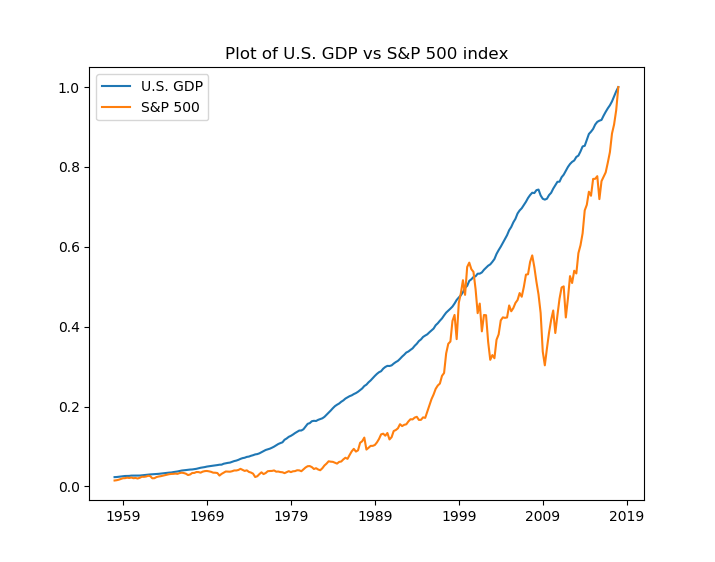
\includegraphics[width=8cm]{GDPvsSP500}
\centering
\caption{Normalised quarterly data from 1958 to 2018 for U.S. GDP and S\&P 500 index. Sources: Standard \& Poor's, U.S. Census Bureau} 
\label{fig:gdpvssp500}
\end{figure}

\subsection{Inflation}
Inflation is the rate at which the general level of prices for goods and services is rising \cite{inflation}. As a result of inflation, the purchasing power of a currency decreases. If the price of milk costs \pounds 1 this year, then with an inflation rate of 2\% it will cost \pounds 1.02 the following year. Central banks define this inflation rate and try to limit inflation, while avoiding deflation, so as to keep the economy running smoothly.    

\subsection{Balance of Trade}
The balance of trade is the difference between the value of a country's imports and exports during a certain period \cite{balanceoftrade}. Economists refer to the balance of trade to measure the relative strength of a country's economy. The balance of trade can be calculated with the following simple formula:

\begin{equation}
    Balance Of Trade = Imports - Exports
\end{equation}

When a country imports more than it exports, it would have a trade deficit, otherwise if it exports more than it imports it would have a trade surplus. A country that has a trade deficit borrows money. This could lead to the value of the country's currency to fall, which will result in consumers paying more for foreign imports \cite{2003economics}. Alternatively a country that has a trade surplus lends money to deficit countries.    

\subsection{GDP}
Historically, GDP (gross domestic product) is one of the most important variables when it comes to measuring the health of an economy. A country's GDP is the total value of all final goods and services produced in the economy \cite{2003economics}. GDP helps define the size of an economy. The bigger the GDP, the more goods are being produced, therefore the healthier the economy is.  There are many factors that effect the GDP such as life expectancy, higher initial schooling, lower inflation and lower fertility \cite{barro1996determinants}. 

\subsection{Unemployment Rate}

The unemployment rate is the percentage of the labour force that is jobless \cite{unemployment}. In a weak economy, jobs tend to be scarce thus the unemployment rate is expected to rise. Alternatively, a healthy economy is more likely that more jobs are available, thus the unemployment rate will decrease. This means that unemployment rate is another factor that highly affects a country's GDP \cite{bean1993unemployment}. A low unemployment rate means that more people are employed and getting paid, which brings in more money into the economy and, as a result, increase GDP.  

\subsection{Interest Rate (Bank Rate)}
In general, the interest rate is a percentage of the amount that one pays when borrowing or gets paid when saving money \cite{interestrate}. If \pounds 1000 is placed into a savings account with a 1\% interest rate, there will be \pounds 1010 the following year.  The bank rate is the most important interest rate in an economy and is set by the central bank. The bank rate is the rate of interest payed on reserves held by commercial banks. Increasing the bank rate makes borrowing more expensive. This means that people will spend less to pay their debts or benefit from better savings rates.



\printbibliography

\end{document}